%!TEX TS-program = pdflatex
%!TEX TS-options = -shell-escape
\RequirePackage{fix-cm}


\newcommand{\obenlinks}{Übungen zur Vorlesung Informatik I}   % hier Name der Veranstaltung eintragen
\documentclass[%
  paper=a4,
  fontsize=10pt,
  ngerman
  ]{scrartcl}

% Basics für Codierung und Sprache
% ===========================================================
  \usepackage{shellesc}                 % Compiler-Option -shell-escape benutzen!
  \usepackage[final]{graphicx}          % Einbindung von Grafiken
  \usepackage{subcaption}
%  \usepackage[utf8]{inputenc}          % Dateien sind UTF8-codiert
  \usepackage{babel}                    % deutsche Silbentrennung, etc.
  \usepackage[german=quotes]{csquotes}  % deutsche Anführungszeichen mit \enquote{...}
% ===========================================================

% Fonts und Typographie
% ===========================================================
  \usepackage[babel=true,final,tracking=smallcaps]{microtype}
  \DisableLigatures{encoding = T1, family = tt* }   % keine Ligaturen für Monospace-Fonts
% ===========================================================

% Farben
% ===========================================================
  \usepackage[usenames,x11names,final]{xcolor}
% ===========================================================

% Mathe-Pakete und -Einstellungen
% ===========================================================
  \usepackage{mathtools}               % Tools zum Setzen von Formeln
  \usepackage{amssymb}                 % übliche Mathe-Symbole
  \usepackage[bigdelims]{newtxmath}    % moderne Mathe-Font
  \allowdisplaybreaks                  % seitenübergreifende Rechnungen
  \usepackage{bm}                      % math bold font
  \usepackage{wasysym}                 % noch mehr Symbole
% ===========================================================

% TikZ
% ===========================================================
  \usepackage{tikz}
  \usetikzlibrary{arrows,arrows.meta}    % mehr Pfeile!
  \usetikzlibrary{calc}                  % TikZ kann rechnen
  \usetikzlibrary{positioning}
  \tikzset{>=Latex}                      % Standard-Pfeilspitze
% ===========================================================

% Seitenlayout, Kopf-/Fußzeile
% ===========================================================
  \usepackage{scrlayer-scrpage}
  \pagestyle{scrheadings}
  \usepackage[top=5cm, bottom=3cm, left=2.5cm, right=2cm]{geometry}
  \clearscrheadfoot 
  \setheadsepline{0.4pt}                            % Linie in Kopfzeile
  \setfootsepline{0.4pt}                            % Linie in Fußzeile
  \setkomafont{section}{\fontsize{14bp}{18.8bp}\normalfont}  % Schriftart der Section
  \setkomafont{subsection}{\fontsize{12bp}{16bp}\normalfont}                  
  \setkomafont{pagehead}{\textnormal}                 % Schriftart Kopfzeile
  \setkomafont{pagefoot}{\normalfont\footnotesize}  % Schriftart Fußzeile 
  \cfoot{\thepage}                                  % Seitenzahl unten Mitte
  \lohead{\obenlinks}                               % Titel oben links
  \raggedbottom                                     % Flattersatz
  \usepackage{setspace}                             % erweiterte Abstandsoptionen
  \onehalfspacing                                   % Zeilenabstand 1.5-fach
  \setlength{\parindent}{0pt}                       % Einrückung neuer Absätze
  \setlength{\parskip}{0.5\baselineskip}            % Abstand neuer Absätze
% ===========================================================

% Hyperref für Referenzen und Hyperlinks
% ===========================================================
  \usepackage[%
    hidelinks,
    pdfpagelabels,
    bookmarksopen=true,
    bookmarksnumbered=true,
    linkcolor=black,
    urlcolor=SkyBlue2,
    plainpages=false,
    pagebackref,
    citecolor=black,
    hypertexnames=true,
    pdfborderstyle={/S/U},
    linkbordercolor=SkyBlue2,
    colorlinks=false,
    backref=false]{hyperref}
  \hypersetup{final}
% ===========================================================

% Listen und Tabellen
% ===========================================================
  \usepackage{multicol}
  \usepackage[shortlabels]{enumitem}
  \setlist{itemsep=0pt}
  \setlist[enumerate]{font=\sffamily\bfseries}
  \setlist[itemize]{label=$\triangleright$}
  \usepackage{tabularx}
% ===========================================================

% minted
% ===========================================================
\usepackage{minted}
\setminted{%
  style=default,
  fontsize=\small,
  breaklines,
  breakanywhere=false,
  breakbytoken=false,
  breakbytokenanywhere=false,
  breakafter={.,},
  autogobble,
  numbersep=3mm,
  tabsize=4,
  linenos,
  frame=lines
}
\setmintedinline{%
  fontsize=\normalsize,
  numbers=none,
  numbersep=12pt,
  tabsize=4,
}

%%%%%%%%%%%%%%%%%%%%%%%%%%%%%%%%%%%%%%%%%%%%%%%%%%%%%%%%%%%
%%% Ab hier folgen nur noch vordefinierte Mathe-Befehle %%%
%%%%%%%%%%%%%%%%%%%%%%%%%%%%%%%%%%%%%%%%%%%%%%%%%%%%%%%%%%%

\newcommand{\BB}{\mathbb{B}}
\newcommand{\CC}{\mathbb{C}}
\newcommand{\NN}{\mathbb{N}}
\newcommand{\QQ}{\mathbb{Q}}
\newcommand{\RR}{\mathbb{R}}
\newcommand{\ZZ}{\mathbb{Z}}
\newcommand{\oh}{\mathcal{O}}            
\newcommand{\ol}[1]{\overline{#1}}
\newcommand{\wt}[1]{\widetilde{#1}}
\newcommand{\wh}[1]{\widehat{#1}}

\DeclareMathOperator{\id}{id}                        % Identität
\DeclareMathOperator{\pot}{\mathcal{P}}              % Potenzmenge

% Klammerungen und ähnliches
\DeclarePairedDelimiter{\absolut}{\lvert}{\rvert}    % Betrag
\DeclarePairedDelimiter{\ceiling}{\lceil}{\rceil}    % aufrunden
\DeclarePairedDelimiter{\Floor}{\lfloor}{\rfloor}    % aufrunden
\DeclarePairedDelimiter{\Norm}{\lVert}{\rVert}       % Norm
\DeclarePairedDelimiter{\sprod}{\langle}{\rangle}    % spitze Klammern
\DeclarePairedDelimiter{\enbrace}{(}{)}              % runde Klammern
\DeclarePairedDelimiter{\benbrace}{\lbrack}{\rbrack} % eckige Klammern
\DeclarePairedDelimiter{\penbrace}{\{}{\}}           % geschweifte Klammern
\newcommand{\Underbrace}[2]{{\underbrace{#1}_{#2}}}  % bessere Unterklammerungen
% Kurzschreibweisen für Faule und Code-Vervollständigung
\newcommand{\abs}[1]{\absolut*{#1}}
\newcommand{\ceil}[1]{\ceiling*{#1}}
\newcommand{\flo}[1]{\Floor*{#1}}
\newcommand{\no}[1]{\Norm*{#1}}
\newcommand{\sk}[1]{\sprod*{#1}}
\newcommand{\enb}[1]{\enbrace*{#1}}
\newcommand{\penb}[1]{\penbrace*{#1}}
\newcommand{\benb}[1]{\benbrace*{#1}}
\newcommand{\stack}[2]{\makebox[1cm][c]{$\stackrel{#1}{#2}$}}  % Präambel (ohne die geht nichts!)
\ihead{
  \section*{Informatik I - Gruppe 1 - Übungblatt 6}
  
  Ausgabe: 14.11.2022

  Abgabe: 21.11.1022

  Tutor: Tim Völker

  ~
}

\ohead{

  ~

  ~

  ~

  Ali Kurt 528961

  Thomas Kujawa 463620

  Felix Hoff 366927

  ~
}


\begin{document}
\graphicspath{ {./images/} }

\textbf{Aufgabe T5.1:} Code verstehen (1+1=2 Punkte )

Sie finden online einen fertigen Programmcode, der wohl etwas hastig geschrieben wurde. Die sehr ineffizient gestaltete Funktion 
wurde wie folgt implementiert:

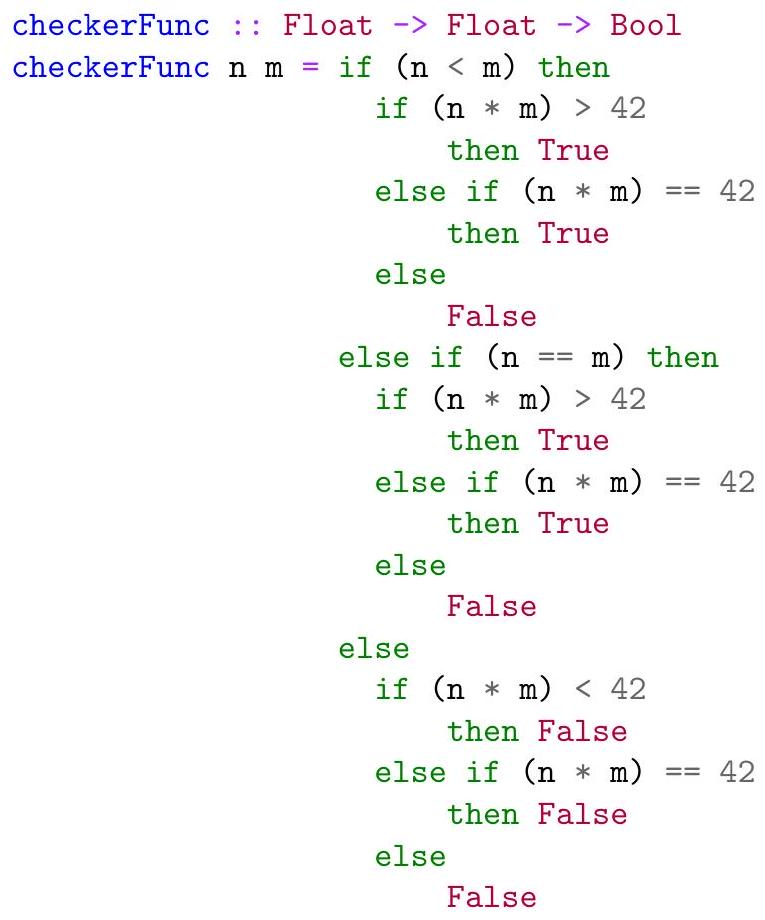
\includegraphics[width=7cm]{2022_11_15_0a5a2eee0aef383b0ce9g-1}

\begin{itemize}
  \item [(a)] Fassen Sie zusammen, welche Eigenschaften von $n$ und $m$ erfüllt sein müssen, damit die Funktion True zurückgibt.

  $(n \le m) \land (n \cdot m \ge 42)$

  \item [(b)] Die Funktion lässt sich in einem einzigen booleschen Ausdruck darstellen. Geben Sie die entsprechende Funktion als 
  Haskellcode (schriftlich) an.

  \inputminted{Haskell}{A5_1.hs}
  
\end{itemize}

$z Z:$ Dic Reihe $\sum_{n=1}^{\infty} a_n$ ist assolut honvergent.
Berris:
Es gilf $q \in \mathbb{R}$ mit $0<q<1$ und $n_0 \geq 0$, sowic $\forall n \geq n_0: \sqrt[n]{\left|a_n\right|} \leq q$
$$
\Leftrightarrow\left|a_n\right| \leq q^n
$$
Dann gitf:
$$
\begin{aligned}
\sum_{n=1}^{\infty}\left|a_n\right| \leq \sum_{n=1}^{\infty} q^n &=\sum_{n=0}^{\infty} q^n-q^0 \\
&(6.4) \frac{1}{1-q}-1=\frac{q}{1-q}<\infty \\
&=\infty
\end{aligned}
$$
Die Reihe $\sum_{n=1}^{\infty} a_n$ honvergint absolut.

\newpage

\textbf{Aufgabe T5.2:} Abgeleitete Klassen (2 Punkte)

In der Vorlesung haben sie Standard-Typklassen wie Ord, Enum oder Num kennengelernt. Im folgenden Programmcode wird ein neuer 
Datentyp Season definiert:

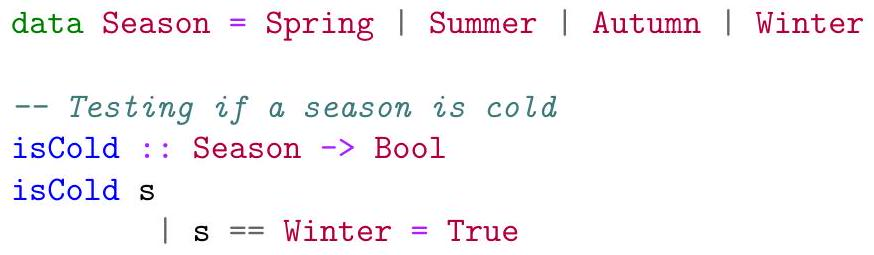
\includegraphics[width=7cm]{2022_11_15_0a5a2eee0aef383b0ce9g-1(1)}

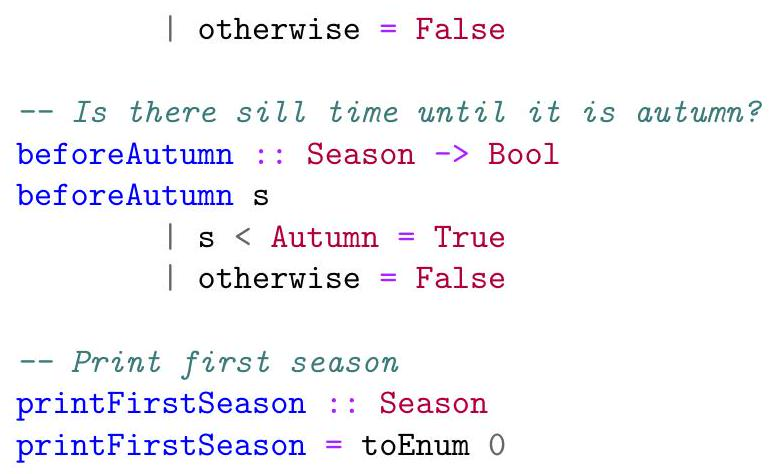
\includegraphics[width=7cm]{2022_11_15_0a5a2eee0aef383b0ce9g-2}

Ausgehend von den gegebenen Funktionen, überprüfen Sie, ob für die neue Klasse alle notwendigen Standard-Typklassen in Form 
einer abgeleiteten Instanzdeklaration angegeben worden sind. Falls nicht, fügen Sie diese noch hinzu und begründen Sie Ihre Antwort.

Hinweis: Verwenden Sie nur die in aus der Vorlesung bekannten Standard-Typklassen.

\newpage

\begin{itemize}
  \item []\inputminted{Haskell}{A5_2.hs}
\end{itemize}

\newpage

\textbf{Aufgabe P5.3:} Klassen $(1+2+5=8$ Punkte $)$

In der Vorlesung wurden die Datentypen Point und Vector umgesetzt. Nun soll eine Klasse Polygon implementiert werden. 
Dabei ist ein Polygon eine Menge von Punkten. Die Klasse Polygon definiert die Funktionen:

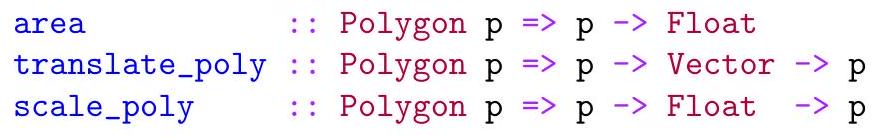
\includegraphics[width=7cm]{2022_11_15_0a5a2eee0aef383b0ce9g-2(1)}

Dabei nimmt die Funktion area ein Polygon entgegen und gibt die Fläche des Polygons zurück. Die Funktion translate 
verschiebt jeden Punkt eines Polygons. Die Verschiebung wird durch einen Vektor angegeben. Die Funktion gibt danach das verschobene 
Polygon zurück. Die Funktion scale multipliziert jeden Punkt eines Polygons mit einer Gleitkommazahl $s$ und gibt das skalierte Polygon 
zurück. Die Ergebnisse aller Funktionen sollen in der Konsole angezeigt werden können. Bearbeiten Sie nun folgende Aufgaben:

\begin{itemize}
  \item [(a)] Implementieren Sie die Datentypen Point und Vector, die Sie in der Vorlesung kennengelernt haben. Dabei sollen die beiden Datentypen keine alternative Schreibweise für Tupel sein, sondern als eigene Datentypen definiert werden. Implementieren Sie die Funktionen translate und scale mit folgender Signatur:

  translate : : Point $\rightarrow$ Vector $\rightarrow$ Point
  
  scale : : Point $\rightarrow$ Float $\rightarrow$ Point
  
  Dabei verschiebt die Funktion translate einen Punkt um einen Vektor und die Funktion scale multipliziert einen Punkt komponentenweise mit einer Gleitkommazahl.

  \item [(b)] Definieren Sie die Klasse Polygon und die Datentypen Triangle (allgemeines Dreieck) und Quad (allgemeines Viereck).

  \item [(c)] Implementieren Sie die Datentypen Triangle und Quad als Instanzen von der Klasse Polygon und implementieren Sie dabei die von der Klasse Polygon definierten Funktionen.

Hinweis: Falls notwendig, recherchieren Sie die Formeln für die benötigten Flächenberechnungen.

\newpage

\inputminted{Haskell}{A5_3.hs}
\end{itemize}

\newpage

\textbf{Aufgabe P5.4:} Aufzählung $(1+2+3=6$ Punkte $)$

Es soll eine Klasse Card für Spielkarten implementiert werden. Eine Spielkarte besteht aus einem Rank (Wert) \{Seven, Eight, Nine, Ten, Jack, Queen, King, Ace\} in aufsteigender Reihenfolge und einem Suit (Farbe) $\{$ Diamond, Heart, Spade, Club $\}$.


\begin{itemize}
  \item [(a)] Implementieren Sie die Datentypen Rank, Suit und Card.

\item [(b)] Implementieren Sie Card als eine Instanz der Klasse Ord. Dabei entscheidet der Wert (Rank) welche Karte größer ist, bei zwei Karten gleichen Wertes entscheidet die Farbe (Suit), welche Karte größer ist. Bei gleichem Wert und gleicher Farbe sind beide Karten gleich groß. 

\item [(c)] Implementieren Sie den Datentypen Hand, der aus drei Karten besteht. Implementieren Sie anschließend eine Funktion value :: Hand $\rightarrow$ Integer, welchen den Wert der Hand zurückgibt. Dabei seien folgende Handkombinationen definiert:

\centering
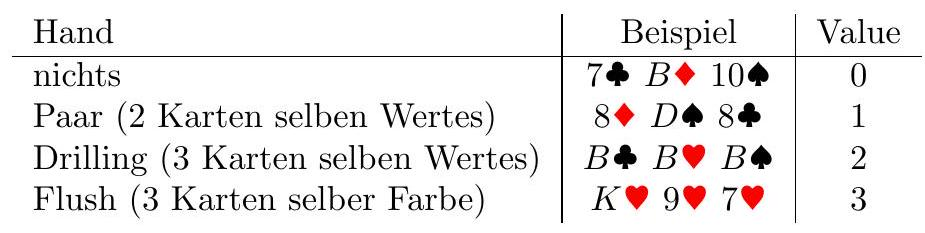
\includegraphics[width=7cm]{2022_11_15_0a5a2eee0aef383b0ce9g-3}

\newpage

\inputminted{Haskell}{A5_4.hs}
\end{itemize}

\newpage

\textbf{Aufgabe P5.5:} Eigene Datentypen $(1+2+2+2=7$ Punkte $)$ 

In dieser Aufgabe sollen Sie einen Datentyp Currency erstellen. Dabei sei eine Currency entweder Euro, Dollar oder Yen. Der Wechselkurs zwischen den verschiedenen Currencies sei dabei:

$$
\begin{aligned}
&1 \text { Dollar }=0,90 \text { Euro } \\
&1 \text { Yen }=0,0083 \text { Euro } \\
&1 \text { Dollar }=108,59 \text { Yen }
\end{aligned}
$$

Bearbeiten Sie hierfür folgende Schritte:

\begin{itemize}
  \item [(a)] Implementieren Sie den Datentyp Currency, der entweder Euro, Dollar oder Yen repräsentiert. Dabei bestehen Euro und Dollar aus zwei Integern für Euro und Cents bzw. Dollar und Cents und Yen besteht nur aus einem Integer.

  \item [(b)] Leiten Sie den Datentyp Currency von der Klasse Show ab und geben Sie Euro und Dollar in der Form 12,03€ bzw. 14,60\$ an und Yen in der Form 120¥. Verwenden Sie hierbei nicht deriving (Show).

  \item [(c)] Schreiben Sie eine Funktion toEuro, die eine Currency entgegennimmt, den entsprechenden Betrag in Euro umrechnet und diesen dann als Currency zurück gibt.

  \item [(d)] Leiten Sie den Datentyp Currency von den Klassen Eq und Ord ab. Beachten Sie dabei, dass verschiedene Currencies verglichen werden können. Verwenden Sie hierbei nicht deriving (Eq, Ord). Geben Sie ein Beispiel als Kommentar an.
  
  \newpage

  \inputminted{Haskell}{A5_5.hs}

\end{itemize}

\end{document}